\documentclass[tikz,border=3mm,multi=tikzpicture]{standalone}
\usepackage{tikz}
\usetikzlibrary{positioning}
\begin{document}
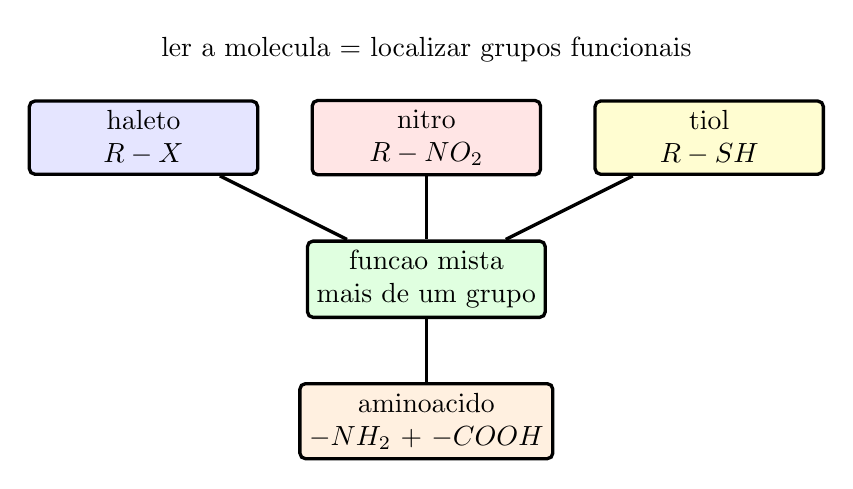
\begin{tikzpicture}[node distance=0.65cm]
  \tikzstyle{box}=[draw,rounded corners=2pt,very thick,minimum width=2.9cm,minimum height=0.8cm,align=center]
  \node[box,fill=blue!10] (hal) {haleto\\$R-X$};
  \node[box,fill=red!10,right=0.65cm of hal] (nitro) {nitro\\$R-NO_2$};
  \node[box,fill=yellow!18,right=0.65cm of nitro] (tiol) {tiol\\$R-SH$};
  \node[box,fill=green!12,below=0.8cm of nitro] (mista) {funcao mista\\mais de um grupo};
  \node[box,fill=orange!12,below=0.8cm of mista] (amino) {aminoacido\\$-NH_2$ + $-COOH$};
  \draw[very thick] (hal) -- (mista);
  \draw[very thick] (nitro) -- (mista);
  \draw[very thick] (tiol) -- (mista);
  \draw[very thick] (mista) -- (amino);
  \node[align=center,above=0.35cm of nitro] {ler a molecula = localizar grupos funcionais};
\end{tikzpicture}
\end{document}
